
\section{One World Rival Theories}
\textcite{snyderOneWorldRival2004}

\begin{center}
    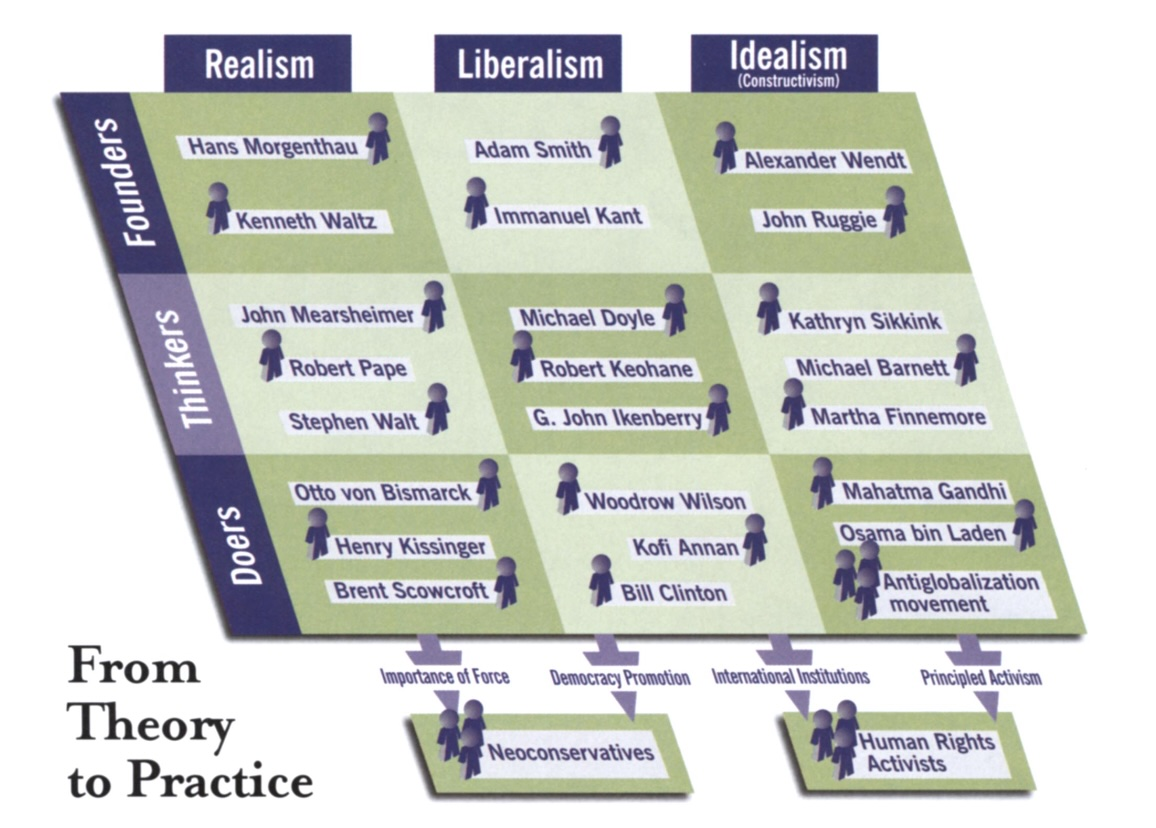
\includegraphics[width=0.7\textwidth]{images/snyder_one_world_rival_theories.jpg}
    \captionof{figure}{\label{fig:fig4_snyder_one_world_rival_theories}%\textit{\parencite[Fig.\(\backsim\)1]{cranmerWhatCanWe2017}}
    }
\end{center}

Realism instills a pragmatic appreciation of the role of power but also warns that states will suffer if they overreach. Liberalism highlights the cooperative potential of mature democracies, especially when working together through effective institutions, but it also notes democracies' tendency to crusade against tyrannies and the propensity of emerging democracies to collapse into violent ethnic turmoil.

Idealism stresses that a consensus on values must underpin any stable political order, yet it also recognizes that forging such a consensus often requires an ideological struggle with the potential for conflict.

It is harder for the normally state-centric realists to explain why the world’s only superpower announced a war against al Qaeda, a nonstate terrorist organization. How can realist theory account for the importance of powerful and violent individuals in a world of states? Realists point out that the

Post-9/11 developments seem to undercut one of realism's core concepts: the balance of power.

When Germany unified in the late 19th century and became Europe's leading military and industrial power, Russia and France (and later, Britain) soon aligned to counter its power. Yet no combination of states or other powers can challenge the United States militarily, and no balancing coalition is imminent.

\subsection{The Divided House of Liberalism}
For its part, the Bush administration highlights democracy promotion while largely turning its back on the international institutions that most liberal theorists champion.

The belief that democracies never fight wars against each other is the closest thing we have to an iron law in social science.

Shortly before September 11, political scientist G. John Ikenberry studied attempts to establish international order by the victors of hegemonic struggles in 1815, 1919, 1945, and 1989. He argued that even the most powerful victor needed to gain the willing cooperation of the vanquished and other weak states by offering a mutually attractive bargain, codified in an international constitutional order.

\begin{center}
    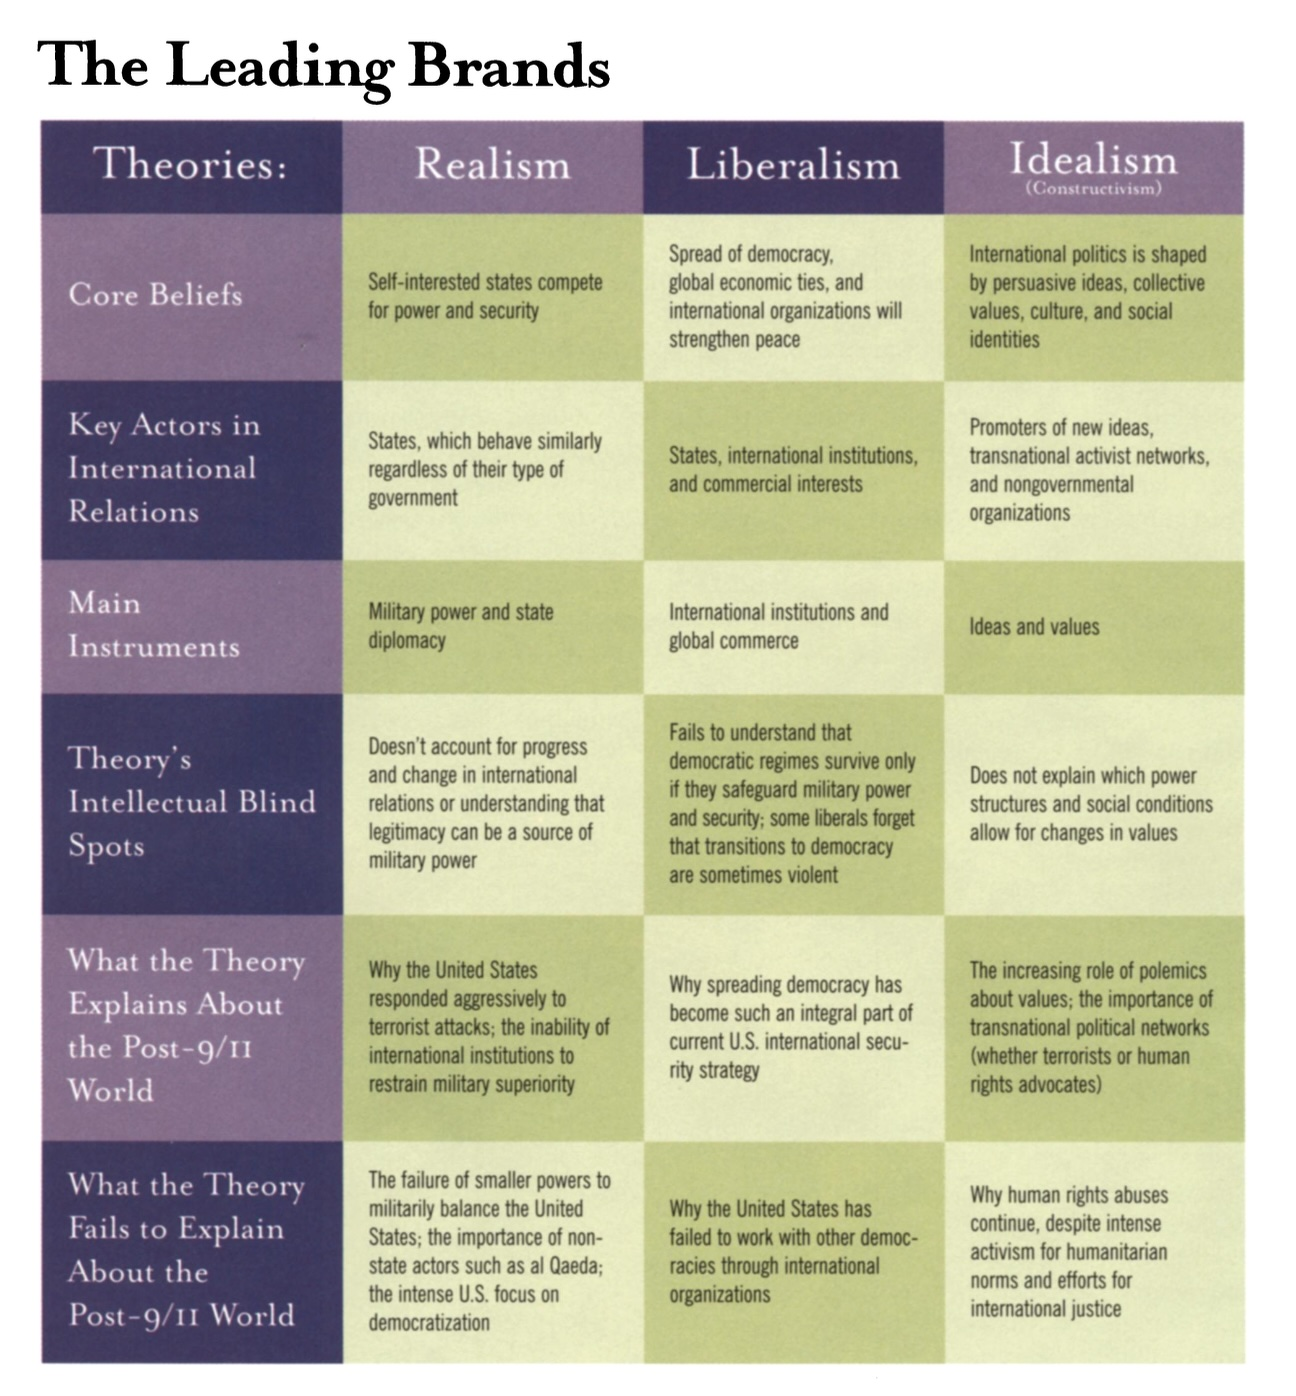
\includegraphics[width=0.7\textwidth]{images/snyder_one_world_rival_theories_the_leading_brands.jpg}
    \captionof{figure}{\label{fig:fig5_snyder_one_world_rival_theories_the_leading_brands}%\textit{\parencite[Fig.\(\backsim\)1]{cranmerWhatCanWe2017}}
    }
\end{center}

\subsection{Idealism}
Idealism: the belief that foreign policy is and should be guided by ethical and legal standards.

\textbf{Constructivism is a new version of idealism:} holds that social reality is created through debate about values, often echoes the themes that human rights and international justice activists sound.

Perhaps most important, Europe’s increasingly legalistic approach to international relations, reflected in the process of forming the European Union out of a collection of sovereign states, provides fertile soil for idealist and constructivist conceptions of international politics.

\textbf{Whereas realists dwell on the balance of power and liberals on the power of international trade and democracy, constructivists believe that debates about ideas are the fundamental building blocks of international life. Individuals and groups become powerful if they can convince others to adopt their ideas.}

Realists failed to predict the end of the Cold War, for example. Even after it happened, they tended to assume that the new system would become multipolar.

Likewise, the liberal theory of democratic peace is stronger on what happens after states become democratic than in predicting the timing of democratic transitions, let alone prescribing how to make transitions happen peacefully.

Constructivists are good at describing changes in norms and ideas, but they are weak on the material and institutional circumstances necessary to support the emergence of consensus about new values and ideas.

With such uncertain guidance from the theoretical realm, it is no wonder that policymakers, activists, and public commentators fall prey to simplistic or wishful thinking about how to effect change.

